
\begin{figure}[ht]
  \centering
  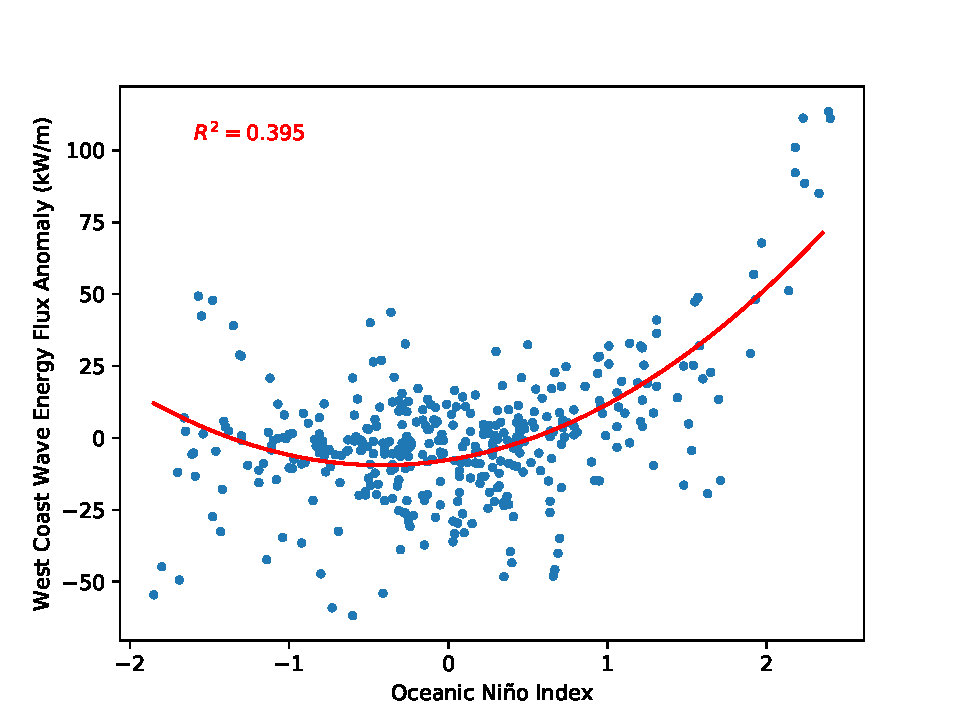
\includegraphics[width=\textwidth]{../fig/ENSO-Comparison.wc.pdf}
  \caption{West Coast wave energy flux anomaly vs. oceanic nino index. The wave energy flux anomaly (annual cycle removed) is averaged along the EEZ boundary, has had a 5-month running average applied, and lags the ONI signal by 2-months.}
  \label{fig:wc-nino}
\end{figure}

\section{Wave Energy Predictability}

One of the main advantages of wave energy is the idea that it is much more predictable than most other renewable energies. On daily to weekly timescales, wave can be predicted by wave propagation models driven be real-time earth observation data-sources (satellites, buoys, etc.).

On inter-annual timescales, several works have noted a correlation with ENSO fluctuations. Figure \ref{fig:wc-nino} compares the West Coast remote wave resource anomaly (the deviation from the annual mean) to the Oceanic Nino Index (ONI) lagged by 2 months. \cite{nationaloceanicandatmosphericadministrationOceanicNinoIndex2020}.
Here we see a strong correlation between the highest values of the west coast resource anomaly and high values of ONI. The fact that the wave resource lags the ONI suggests that the ONI can be used to predict peaks in wave energy. This correlation is likely to be causal because ENSO events are correlated with larger storms in the S. Pacific, which is a major source of wave energy on the U.S. West Coast \citep{andersonClimateIndexOptimized2018, yangCharacteristicsVariabilityNearshore2020, ruggieroNationalAssessmentShoreline2013}.

On shorter timescales, modern improvements in wave modeling have made significant advances in the accuracy of wave prediction \citep{cavaleriWaveModellingCoastal2018}. Applications of artificial intelligence have also shown promise for accurate prediction of wave height and wave power \citep[e.g.][]{cornejo-bueno_significant_2016}. This predictability, and the degree to which wave energy compliments other types of renewable energy in specific locations, may become increasingly valuable as electrical grids are powered increasingly by variable renewables \cite{parkinsonIntegratingOceanWave2015}.



\section{Summary} \label{sec:conclusion}

We propose a methodology for theoretical wave resource assessment that resolves several outstanding issues with earlier approaches. In particular, this work accounts for wave directionality in order to reduce `double counting', and also includes the energy added to the wave field by local winds. This provides a consistent methodology for accounting for wave energy at national/regional scales. So that policy makers can have a clear understanding of wave energy potential. As other nations/regions adopt the methodology, we will have an apples-to-apples comparison of opportunity, which can inform decision making and investment.

We then apply this methodology to the U.S. EEZ (except for the portion of the EEZ associated with U.S. Pacific Islands Territories), and find that the total U.S. wave energy resource is greater than 3,300 TWh/yr.
This is an increase of ~25\% compared to earlier DOE wave resource assessments, and is due to the combination of extending the resource area to the edge of the EEZ and incorporating the local resource. The `inner shelf' resource (i.e., at 10 nautical-miles from shore) is estimated herein to be 1800 TWh/yr.

A detailed assessment of the ``technical resource potential'', which accounts for the efficiency and array design of existing technologies is left for future work. Furthermore, an assessment of the ``practical resource'' is a greater challenge because it requires accounting for regional permitting details, ocean-planning designations, and competing uses by other ocean stakeholders.

The methodology proposed in this study demonstrates the importance of including local resource to accurately assess the total theoretical resources at regional scales. It would benefit the wave energy community if this methodology were incorporated into IEC standards so that there is clarity and consistency on these types of assessments. Furthermore, the methods proposed here could also be of use to project developers in identifying the maximum resource potential of a project site.

%\subsection{SOME EXTRA TEXT FROM DISCUSSION}

%Will devices of the future be sufficiently broad-banded to extract the local resource and remote resource equally efficiently? 
%What technological changes are required to make that happen? There is use for this energy in niche blue economy markets, or if energy storage technologies (e.g., liquid renewable fuels) become sufficiently inexpensive. If so, will the WEC technologies be economically competitive? 

%%% Local Variables:
%%% TeX-master: "wave_res"
%%% End:
